% Options for packages loaded elsewhere
\PassOptionsToPackage{unicode}{hyperref}
\PassOptionsToPackage{hyphens}{url}
\PassOptionsToPackage{dvipsnames,svgnames,x11names}{xcolor}
%
\documentclass[
  10pt,
]{article}
\usepackage{amsmath,amssymb}
\usepackage{iftex}
\ifPDFTeX
  \usepackage[T1]{fontenc}
  \usepackage[utf8]{inputenc}
  \usepackage{textcomp} % provide euro and other symbols
\else % if luatex or xetex
  \usepackage{unicode-math} % this also loads fontspec
  \defaultfontfeatures{Scale=MatchLowercase}
  \defaultfontfeatures[\rmfamily]{Ligatures=TeX,Scale=1}
\fi
\usepackage{lmodern}
\ifPDFTeX\else
  % xetex/luatex font selection
\fi
% Use upquote if available, for straight quotes in verbatim environments
\IfFileExists{upquote.sty}{\usepackage{upquote}}{}
\IfFileExists{microtype.sty}{% use microtype if available
  \usepackage[]{microtype}
  \UseMicrotypeSet[protrusion]{basicmath} % disable protrusion for tt fonts
}{}
\makeatletter
\@ifundefined{KOMAClassName}{% if non-KOMA class
  \IfFileExists{parskip.sty}{%
    \usepackage{parskip}
  }{% else
    \setlength{\parindent}{0pt}
    \setlength{\parskip}{6pt plus 2pt minus 1pt}}
}{% if KOMA class
  \KOMAoptions{parskip=half}}
\makeatother
\usepackage{xcolor}
\usepackage[margin=22mm]{geometry}
\usepackage{longtable,booktabs,array}
\usepackage{calc} % for calculating minipage widths
% Correct order of tables after \paragraph or \subparagraph
\usepackage{etoolbox}
\makeatletter
\patchcmd\longtable{\par}{\if@noskipsec\mbox{}\fi\par}{}{}
\makeatother
% Allow footnotes in longtable head/foot
\IfFileExists{footnotehyper.sty}{\usepackage{footnotehyper}}{\usepackage{footnote}}
\makesavenoteenv{longtable}
\usepackage{graphicx}
\makeatletter
\def\maxwidth{\ifdim\Gin@nat@width>\linewidth\linewidth\else\Gin@nat@width\fi}
\def\maxheight{\ifdim\Gin@nat@height>\textheight\textheight\else\Gin@nat@height\fi}
\makeatother
% Scale images if necessary, so that they will not overflow the page
% margins by default, and it is still possible to overwrite the defaults
% using explicit options in \includegraphics[width, height, ...]{}
\setkeys{Gin}{width=\maxwidth,height=\maxheight,keepaspectratio}
% Set default figure placement to htbp
\makeatletter
\def\fps@figure{htbp}
\makeatother
\setlength{\emergencystretch}{3em} % prevent overfull lines
\providecommand{\tightlist}{%
  \setlength{\itemsep}{0pt}\setlength{\parskip}{0pt}}
\setcounter{secnumdepth}{-\maxdimen} % remove section numbering
\ifLuaTeX
  \usepackage{selnolig}  % disable illegal ligatures
\fi
\usepackage{bookmark}
\IfFileExists{xurl.sty}{\usepackage{xurl}}{} % add URL line breaks if available
\urlstyle{same}
\hypersetup{
  colorlinks=true,
  linkcolor={Maroon},
  filecolor={Maroon},
  citecolor={Blue},
  urlcolor={blue},
  pdfcreator={LaTeX via pandoc}}

\author{}
\date{}

\begin{document}

\section{APS: four lead implementations and an instruction
audit}\label{aps-four-lead-implementations-and-an-instruction-audit}

This continuation implements the four proposals from
\href{../aps_leads_20261105/README.md}{the lead report}, exposes them
under the new \texttt{ic.aps\_v3} identity, and extends the separate
ordinary-residue reader. Development observations have producer
standing, \textbf{unverified}; they are not benchmark data or a signed
PCC verdict {[}pcc:unverified{]}.

Deliverables: \href{pipeline.dot}{editable diagram},
\href{report.pdf}{report PDF}, \href{PROOFS.md}{proof map},
\href{ACCOUNTING.md}{cost contract}, and \href{PROTOCOL.md}{design
draft}.

\begin{longtable}[]{@{}
  >{\raggedright\arraybackslash}p{(\columnwidth - 4\tabcolsep) * \real{0.3333}}
  >{\raggedright\arraybackslash}p{(\columnwidth - 4\tabcolsep) * \real{0.3333}}
  >{\raggedright\arraybackslash}p{(\columnwidth - 4\tabcolsep) * \real{0.3333}}@{}}
\toprule\noalign{}
\begin{minipage}[b]{\linewidth}\raggedright
Requested step
\end{minipage} & \begin{minipage}[b]{\linewidth}\raggedright
Delivered component
\end{minipage} & \begin{minipage}[b]{\linewidth}\raggedright
Still required
\end{minipage} \\
\midrule\noalign{}
\endhead
\bottomrule\noalign{}
\endlastfoot
1. Measurement readiness & Explicit lead controls; literal
cells/history; separate arithmetic/full-set reader; optional
method-plus-scalar Ir reconstruction & Actual profile/metric admission,
complete GAE pricing, pilot, fixed analysis and frozen main protocol \\
2. Approved source checkpoint & Approval preserved; source-only GitHub
gate and pinned selection support prepared & Fresh fenced admission,
actual existing secret binding and successful standard gate; preparing
code is not an upload \\
3. Baseline measurements & Original comparisons and four-size workload
requirement retained in \texttt{PROTOCOL.md} & Successful prerequisites
and actual EKS pilot/main execution; no performance numbers supplied \\
4. Implement and compare leads & Native trace pool, two-variable line
chart, unequal profiles/arbitrary guesses, retained-base full/frontier
controls and separate reader & Admitted measured comparisons;
development tests do not establish improvement \\
\end{longtable}

\subsection{Implementation}\label{implementation}

\begin{itemize}
\tightlist
\item
  \textbf{Trace reuse:} each target starts with an empty bounded pool.
  Existing native F4 record/replay supplies the candidate basis;
  numerical input reductions and every Buchberger S-pair must reduce to
  zero. An invalid, mismatched or resource-capped candidate falls back
  to ordinary F4. Learning, replay, checking, fallback and retained
  trace words remain visible.
\item
  \textbf{Line chart:} for \(y=tx+c\), use \(U=t^2\), \(V=c/t\) when
  \(t\ne0\). The divisor coefficients become \(e_1=U\), \(e_2=a-2UV\),
  \(e_3=UV^2-b\). The chart uses two unknowns; a separate one-variable
  horizontal cell is retained unless the existing propagated-orbit label
  certificate allows omission. Ordinate-zero and zero-denominator cases
  are refused. The existing unpruned line formulation also uses two
  variables. The certified pruned formulation uses a third inverse
  variable, which this chart removes; the protocol distinguishes these
  two comparisons.
\item
  \textbf{Profiles and elimination:} original partition sizes are
  explicit, bounded and may differ. Guess any original coordinate before
  F4 and restore it before relation recovery. No unknown logarithm is
  supplied to a solver.
\item
  \textbf{Growth:} preserve points and labels, append conditional new
  draws, and keep partial sampling failures. \texttt{retained\_full} and
  \texttt{frontier} share the same nested base law. The latter skips old
  tuples only after a complete, non-timeout, non-early-stop traversal
  without an informative witness.
\end{itemize}

The implementations are bounded development backends: prime fields up to
65,521, arity three/four, original partition sizes one through four,
degree bound at most 24 and explicit finite attempt/draw/time budgets.
Cubic orbit expansion uses its existing independent certificate. No cap
is lifted here. The existing six encodings and frozen v1/v2 records
retain their behavior.

The independent reader validates actual producer records using ordinary
residue affine arithmetic. It checks the partition/guess/chart cell
geometry, literal digests, retained labels/draw totals, trace counter
continuity and complete root sets through finite point combinations. A
complete frontier's expected set is the new product's solutions minus
the certified old product's solutions. A partial report only supports
subset checking. This is separate software, not signed execution or
raw-profile authenticity {[}pcc:unverified{]}.

\subsection{Cost and formal
boundaries}\label{cost-and-formal-boundaries}

\url{ACCOUNTING.md} defines optional inclusive Ir evidence and the
excluded work. All operation-cost/execution flags remain honest: native
GAE totals are incomplete; an unkeyed receipt is not execution proof.
The new frame reader does not turn test duration into timing evidence.

\url{PROOFS.md} supplies the mathematical argument and proof map. The
central frontier cover/disjointness statement has a core-only Lean
formalization. Chart lifting into actual finite-field curve relations
and the implementation-to-proof refinement remain open. The previous
native identity records are reused at their original scope, never
treated as PCC solve certificates or full chart-completeness proofs
{[}pcc:unverified{]}.

\url{PROTOCOL.md} is a design continuation, \textbf{not a freeze}. It
keeps the original baseline comparisons, four held-out size classes,
same-input references, controls, failures and complete cold-cost
obligations. The source checkpoint is approved; local authentication is
not bound and the repository secret path has not yet produced a gate
outcome. No benchmark, runtime pilot, profiler run or EKS experiment was
launched.

\subsection{Evidence and continuation}\label{evidence-and-continuation}

\url{SOURCE_CHECKPOINT.md} describes a checkpoint-only GitHub path using
the repository's existing secret reference. It requires a fresh T10
fence, exact source selection and a bounded upload window. Preparing
that path is not a source upload, a gate pass or a benchmark admission.

\texttt{validation/early-boundaries.json} preserves the earlier failed
and superseded development observations under native claim
\texttt{PCC-20261106-e8b5a4}, standing \textbf{unverified}. It
explicitly does not pin a complete source tree for those earlier
commands. Final source-linked receipts will be additive; no earlier
boundary becomes a final full-suite pass. Raw dependency/build/host logs
and the native full ledger stay private.

\href{validation/focused-checks.json}{Focused checks} pin their actual
source boundaries. Native statement \texttt{PCC-20261106-cc59ba} records
the public lead, producer/reader and example observations, plus the
separate standalone export boundary. Its standing is
\textbf{unverified}; the root-library outcome and later reader-overflow
hardening have their own continuation receipts {[}pcc:unverified{]}.
Native statement \texttt{PCC-20261106-34db73} pins
\href{validation/completed-components.json}{completed component checks},
including the seven-test boundary before the later native-session test.
Registry and optimization-policy repairs have their own subsequent
validation; no earlier pass is transferred to them {[}pcc:unverified{]}.

The subsequent \href{validation/final-components.json}{final component
receipt}, native statement \texttt{PCC-20261106-5e324a}, records eight
public lead tests, the existing producer bridges and examples, the
repaired registry and optimization inventory, focused units and strict
Rust 1.98/stable lints. Its standing is \textbf{unverified}. The native
scratch session is a correctness check; APS receives a static audit and
the rho control alone receives count replay. The broad library command
remains a separate, earlier source boundary with failures and no final
verdict in this receipt {[}pcc:unverified{]}. See \url{CHECKS.md} for
the exact boundaries and limitations.

The algorithm/reader source-only pin is
\href{https://github.com/isogeny-labs/crypto/commit/413a93d6f9940c855200468175174126136bb49c}{\texttt{413a93d6f9940c855200468175174126136bb49c}}.
See the
\href{https://github.com/isogeny-labs/crypto/blob/413a93d6f9940c855200468175174126136bb49c/src/cryptanalysis/aps_single_relation/leads.rs}{lead
cells},
\href{https://github.com/isogeny-labs/crypto/blob/413a93d6f9940c855200468175174126136bb49c/src/cryptanalysis/f4_fp/reuse.rs}{trace
pool},
\href{https://github.com/isogeny-labs/crypto/blob/413a93d6f9940c855200468175174126136bb49c/tests/aps_cost_leads.rs}{public
producer bridge} and
\href{https://github.com/isogeny-labs/crypto/blob/413a93d6f9940c855200468175174126136bb49c/tools/aps-export/src/inclusive.rs}{inclusive
reader}. These links pin source, not an execution or performance
verdict.

\url{HANDOFF.md} tracks the unfinished work. T9/research and
T10/authblocked checkpoint stay open. Passing development tests or a
merged implementation PR does not discharge the baseline/scaling
request.

Sources checked: Amadori--Pintore--Sala,
\href{https://iris.unitn.it/retrieve/e3835194-60e8-72ef-e053-3705fe0ad821/Amadori\%2C\%20Pintore\%2C\%20Sala\%20-\%20On\%20DLP\%20for\%20prime-field\%20EC\%20\%28rev\%29.pdf}{revised
manuscript}, sections 3.1--3.3; the
\href{../aps_leads_20261105/SOURCES.md}{previous source map}, existing
F4 record/replay, existing unequal-profile sampler and existing native
Callgrind parser. KB unavailable: no loaded KB tool or local indexed
runtime/catalog; the fallback is these primary and repository sources.
No novelty claim.

Canonical scoreboard/curve/performance diagrams have no new measured
value to add; they remain unchanged. This study supplies its own
implementation and admission diagram and source-linked report, without a
performance plot.

\begin{figure}
\centering
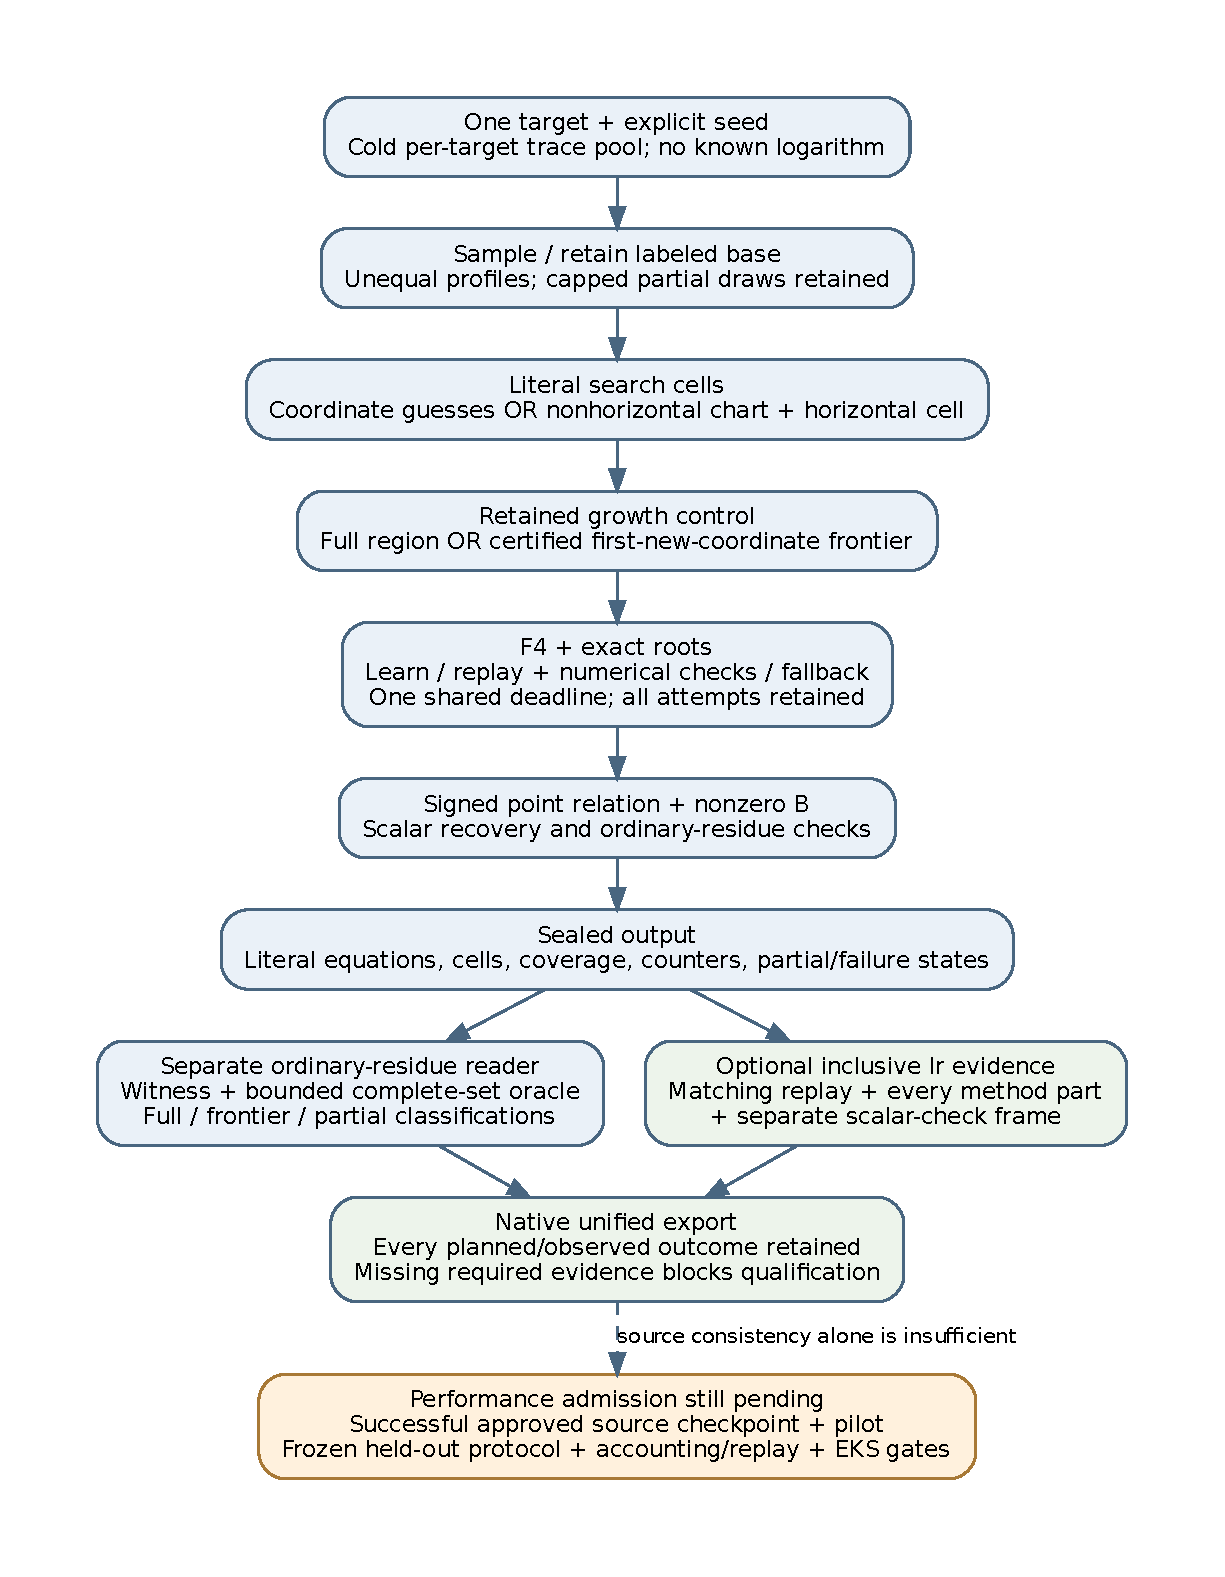
\includegraphics{pipeline.pdf}
\caption{Implemented search paths and pending measurement admission}
\end{figure}

\end{document}
